\chapter{Numerical Results}
\label{Numerical Results}

In this chapter, we  present some numerical studies concerning simulations with the RWM algorithm and the MALA algorithm. A simple simulation tool has been implemented in python and has been used to generate the following figures. We  briefly describe some properties like the estimation of integrated autocorrelation time to avoid ambiguousness. Also the different target distributions are described which have been used for the simulations. Mainly, we want to verify that the theoretical and asymptotical results hold for finite dimensions~$N$. This has been reached by performing simulations with RWM and MALA having been applied to several target distributions. Afterwards, these simulations have been analyzed to measure the complexity and to find the optimal scaling (of the proposal variance) depending on $N$.
Further numerical studies concerning the optimal scaling of Metropolis-Hastings methods, and in particular the RWM and MALA algorithm, can be found in~\autocite{Beskos2008, Gelman1996, Roberts2001}.

\section{Measuring Complexity}
\label{NR- autocorrelation time}

In this section, we briefly present the used measure of complexity. As introduced in Chapter~\ref{CC:Criteria}, there exist no uniqe and best criteria to ascertain a good performance of a time-discrete Markov chain and hence, a Metropolis-Hastings method. We  introduce the \textit{autocorrelation time}, or more precisely, an suitable estimator for this quantity and related estimators as the \textit{standard error of the mean}. The theory for these estimators is taken from~\autocite{Geyer1992}.


%\section{Implementation in Python}



\section{Numerical Simulations}

In this section, we present three selected numerical studies concerning Metropolis-Hastings methods. We try to answer three questions: 
\begin{enumerate}
 \item How do the RWM and MALA algorithms behave in high dimensions for a nonproduct target distribution? Do the observations coincide with the theory developed in Chapter~\ref{Diffusion Limit Results}?
 \item Do the theoretical results in Chapter~\ref{ch:Computational Complexity} and~\ref{Diffusion Limit Results} apply for small dimension~$N$? 
 \item Can we quantify a significantly better performance of the MALA algorithm compared to the RWM algorithm in practice? 
\end{enumerate}

To answer these three questions, we did several numerical studies for different target distributions. In the following, we present for each of these three questions concerning the performance of RWM and MALA algorithms in different dimensions, the result of our simulations. As the results for each question are similar for different target distributions, we illustrate each study applied to a different target measure~$\pi^N$.


\subsection{RWM and MALA Applied to Non-product Targets in Various Dimensions}
\label{sec:sub:Numericals Non-product targets}

\begin{figure}%[htb]
 \begin{center} 
  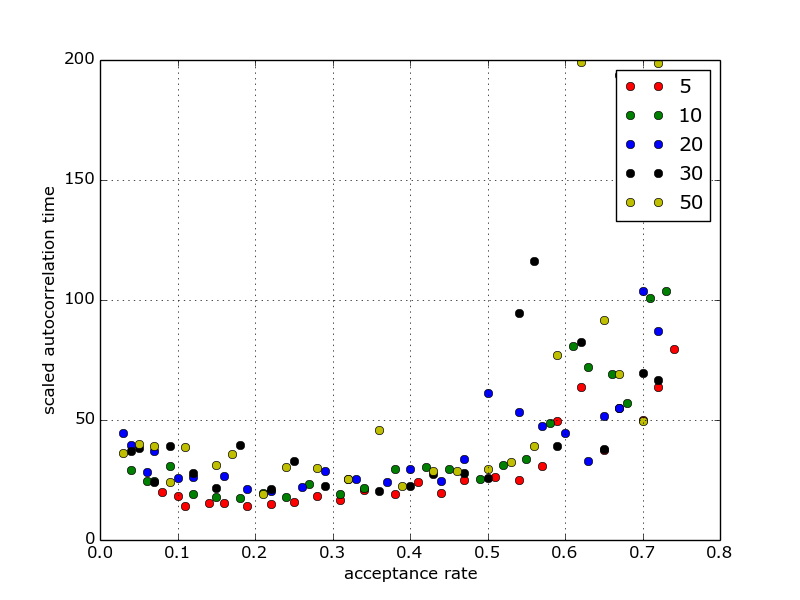
\includegraphics[width=0.83\textwidth]{RWM_ScaledAutocorrelationsDiagramm_MultimodalGaussian-m=2}
  \vspace*{1mm}
  \subcaption{The optimal scaling of RWM methods is achieved for acceptance rates near 0.234.}
  \label{fig:OptimalScaling-RWM-dimensions}
  \vspace*{3mm}
  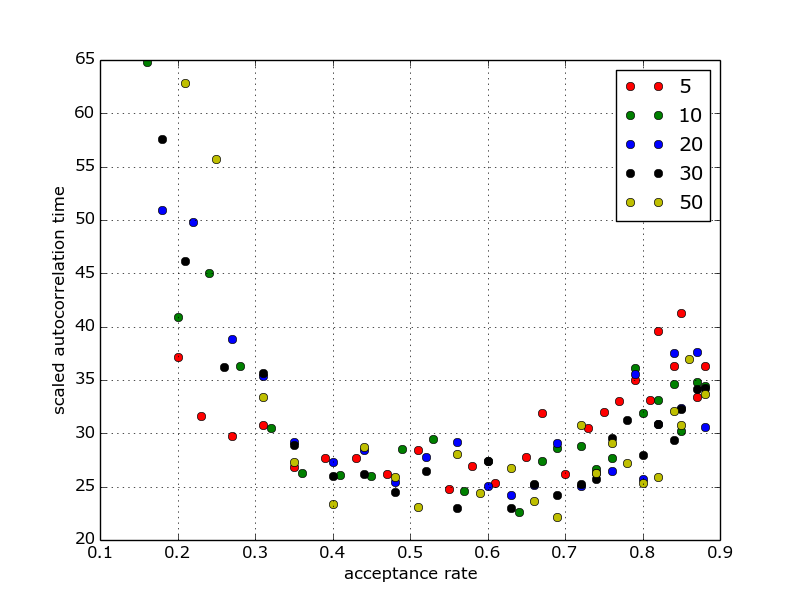
\includegraphics[width=0.83\textwidth]{MALA_ScaledAutocorrelationsDiagramm_MultimodalGaussian-m=2}
  \vspace*{1mm}
  \subcaption{The optimal scaling of MALA methods is achieved for acceptance rates near 0.574.}
  \label{fig:OptimalScaling-MALA-dimensions}
 \end{center}
  \caption{Plotted scaled autocorrelation time for different acceptance rates and various dimensions for the multimodal Gaussian target given in Equation~(\ref{NR-multimodal}).}
  \label{fig:OptimalScaling for RWM and MALA in various dimensions}
\end{figure}

For instance, consider a $N$-dimensional bimodal target density of the form
\begin{equation}
 \label{NR-multimodal}
 \pi^{N} = \tfrac{1}{2} \; \mathcal{N}(-\mu_N, I_N ) +  \tfrac{1}{2} \; \mathcal{N}(\mu_N, I_N ),
\end{equation}
where $\mu_N = (m_N, 0, \dots, 0) \in \mathbb{R}^N$. The mass of this distribution is centered in the two modes~$-\mu_N$ and $\mu_N$. Although, this is the sum of two simple $N$-dimensional Gaussians, the bimodal distribution is neiher of i.i.d.\,product form nor of a scaled product form as defined in Equations~(\ref{CC:iid product targets} and~(\ref{CC:Scaled product targets}), respectively. Indeed, the first coordinate is not merely a rescaling of the other coordinates. 


A numerical study for $m_N = 2$ for the RWM and MALA method is illustrated in Figure~\ref{fig:OptimalScaling for RWM and MALA in various dimensions}. For each dimension $N \in \{ 5, 10, 20, 30, 50 \}$, several simulations of the RWM and MALA algorithm applied to the target defined in Equation~(\ref{NR-multimodal}) are performed. For different average acceptance rates, the scaled integrated autocorrelation time is calculated according to Section~\ref{NR- autocorrelation time}. In the case of the RWM method, the integrated autocorrelation time is scaled by a factor of~$N^{-1}$.  For each single dimension~$N$, the scaled integrated autocorrelation times approximately form a flat and quadratic ``curve'' with its minimum around 0.25. For high acceptance rates and large dimensions, the variance of the estimator for the integrated autocorrelation time increases such that these samples are more scattered than the others. Nevertheless, for the scaling~$N^{-1}$ these different curves ``converge'' in the sense that they lie on above the other. Therfore, the theoretical optimal scaling of~$\mathcal{O}(N)$ for the RWM algorithm obtained in Theorem~\ref{DLR-THM main theorem} seems reasonable. For the MALA algorithm, we obtain similar results with a scaling of~$N^{-1/3}$. In contrast, the ``curves'' for the MALA simulations have their minima near 0.6 and for low acceptance rates, the performance for all dimensions is worse. However, the integrated autocorrelation times of the MALA algorithm are in total smaller than the analogue times of the RWM algorithm. Several facts are well illustrated by Figure~\ref{fig:OptimalScaling for RWM and MALA in various dimensions}:
\begin{enumerate}
 \item Best performance of RWM near an acceptance rate of 0.234 and of MALA near an acceptance rate of 0.573. Hence, asymptotic results seem to apply for finite dimensional setting ($N \geq 5$).
 \item To reach optimality, it suffices to scale the simulation such that the average acceptance rate is near the optimal values of 0.234 and 0.574. The performance of RWM is good for an average acceptance rate in the intervall $[0.1, 0.4]$ and the MALA performs well for $[0.4, 0.75]$.
 \item It is not surprising, that the MALA algorithm  in practice has a lower scaled integrated autocorrelation time as the theoretical complexity is better in comparison to the RWM algorithm due to the gradient information in the proposal of MALA algorithm.
\end{enumerate}

\begin{rem}
 The gradient~$\nabla \log \pi^{N}$ in the MALA algorithm can be numerically approximated by finite differences. Moreover, for both methods, a parallelization for high dimensions is possible. As only the acceptance and rejection steps require all information on the actual position and the possible candidate, a spreading of information once per iteration is sufficient.
\end{rem}


\subsection{Validity in Low Dimensions}
\label{sub:sec:Numericals Low dimensions}

Consider a simple multidimensional Gaussian distribution in $\mathbb{R}^N$  of the form
\begin{equation}
 \label{Numerical: Definition standard Gaussian}
 \pi^N (x) \varpropto \exp \left( -\tfrac{1}{2} \langle x - \mu^N, (\Sigma^N)^{-1} (x-\mu^N) \rangle  \right),
\end{equation}
with covariance matrix~$\Sigma^N = \sigma^2 I_N$ for $\sigma^2 >0$ and mean~$\mu^N = (0, \dots, 0)^T$. This distribution can be represented as a product of i.i.d.\,components, hence, Theorem~\ref{CC: Product Diffusion Limit Result} can be applied and states that the optimal scaling for the RWM algorithm is $\mathcal{O}(N)$ with an optimal acceptance rate of 0.234 and for MALA algorithm, the optimal scaling is $\mathcal{O}(N^{1/3})$ with an optimal acceptance rate 0f 0.574. This result is asymptotical for dimension~$N$ going to infinity. Hence, we wonder if this optimality results apply to finite dimensions. To answer this question, we did several simulations for the standard Gaussian distribution given in Equation~(\ref{Numerical: Definition standard Gaussian}) in small dimensions~$N \in \{ 1,2,3,4,5,8,10 \}$ for different acceptance rates. For each simulation, the scaled autocorrelation time as introduced in Section~\ref{NR- autocorrelation time} was estimated. The result is illustrated in Figure~\ref{fig:OptimalScaling for RWM and MALA in small dimensions}. It seems that only for dimension~$N=1$, the optimal acceptance rate is significantly higher than in the general asymptotic case. From dimension~$N=2$ for the MALA algorithm or $N=3$ for the RWM algorithm, the rule of thumb to tune the acceptance rate apply in this numerical study. Thus, it seems that the asymptotic results obtained by diffusion limits apply to finite dimensions and even to small dimensions larger than $N=3$. 

\begin{figure}%[htb]
 \begin{center} 
  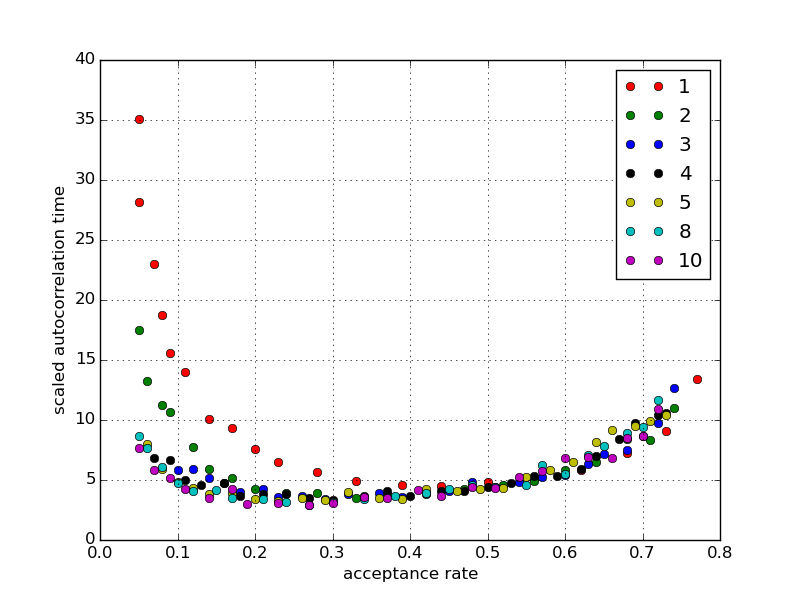
\includegraphics[width=0.8\textwidth]{RWM_convergenceDiagramm_2}
  \vspace*{1mm}
  \subcaption{The optimal scaling of RWM methods is achieved for acceptance rates near 0.234 for dimensions larger than $N=3$.}
  \label{fig:OptimalScaling-RWM-small-dimensions}
  \vspace*{3mm}
  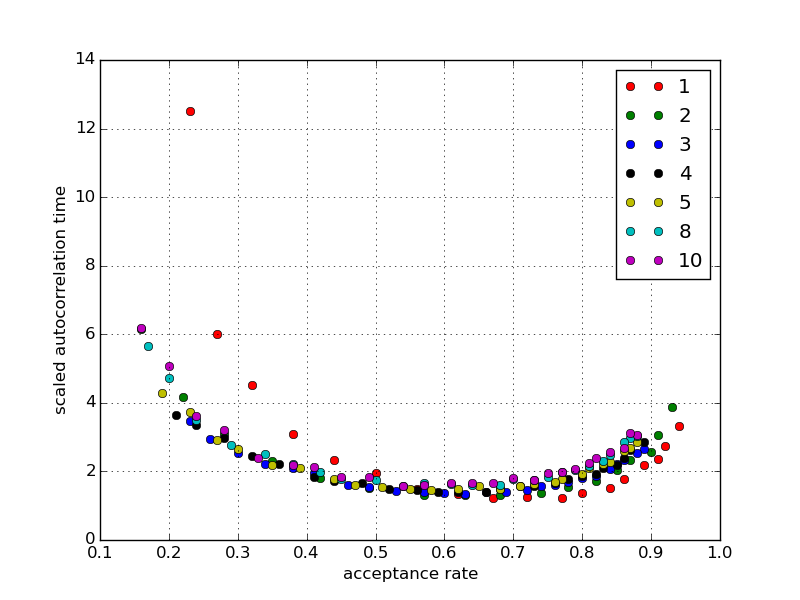
\includegraphics[width=0.8\textwidth]{MALA_convergenceDiagramm_2}
  \vspace*{1mm}
  \subcaption{The optimal scaling of MALA methods is achieved for acceptance rates near 0.574 for dimensions larger than $N=2$.}
  \label{fig:OptimalScaling-MALA-small-dimensions}
 \end{center}
  \caption{Plotted scaled autocorrelation time for different acceptance rates and small dimensions for the standard Gaussian target given in Equation~(\ref{Numerical: Definition standard Gaussian}).}
  \label{fig:OptimalScaling for RWM and MALA in small dimensions}
\end{figure}


\subsection{Comparison of the Performance of RWM and MALA Algorithm}
\label{sec:sub:Numericals: Comparison MALA - RWM}

To compare the performance of MALA and RWM algorithm, we chose the target distribution~$\pi^N$ of the form
\begin{equation}
 \label{Numerical: Definition: Changed Gaussian}
 \pi^N (x) \varpropto \exp \left(- \tfrac{1}{2} \| x \|_{\mathcal{C}^N}^2 - \Psi^N (x) \right)
\end{equation}
with
\begin{equation}
 \label{Numerical: Definition: Psi^N and C^N}
 \| x \|_{\mathcal{C}^N}^2 := \langle x, (\mathcal{C}^N)^{-1}x \rangle = \sum_{j=1}^N \lambda_j^2 x_j^2, \qquad \Psi^N (x) := \tfrac{1}{2} \|P^N x \|^2_{s}=\tfrac{1}{2} \sum_{j=1}^{N} j^{2s}x_j^2.
\end{equation}
Here, we used the notation introduced in Chapter~\ref{sec:DLR-Preliminaries}. By choosing $\mathcal{C}^N := \sigma^2 I_N$, where $I_N$ is the identity in dimension~$N$ and $\sigma^2>0$, we obtain the following representation of~$\pi^N$ in its coordinate form
\begin{equation}
\label{Numericla: Definition: Changed Gaussian coordinates}
 \pi^N (x) \varpropto \exp \left( -\tfrac{1}{2} \sum_{j=1}^N ( \sigma^{-2} + j^{2s}) x_j^2   \right).
\end{equation}

\begin{figure}%[htb]
 \begin{center} 
  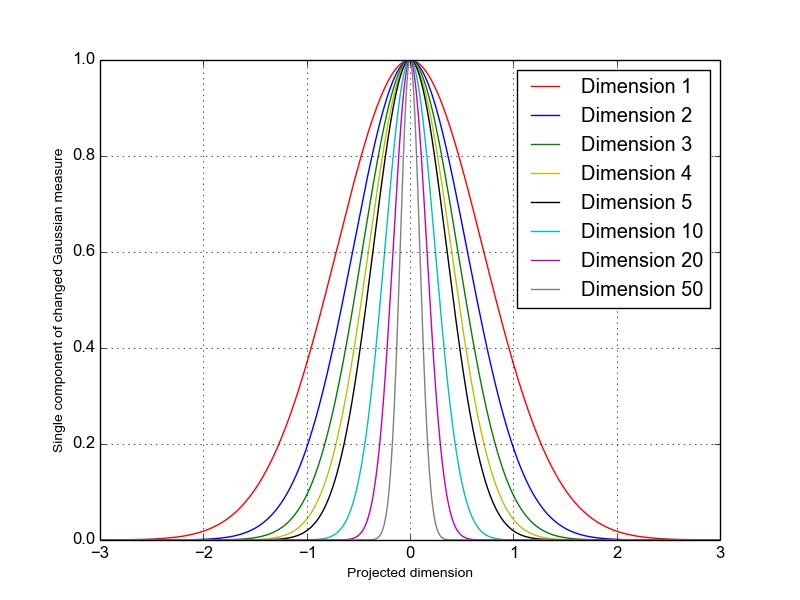
\includegraphics[width=0.60\textwidth]{figure_ChangedGaussian}
 \end{center}
  \caption{Plot of the different dimensions of the changed Gaussian given in Equation~(\ref{Numericla: Definition: Changed Gaussian coordinates}) with $\sigma^2 = 1.0$ and $s = 1.0$.}
  \label{fig:target: Changed Gaussian}
\end{figure}

In~\autocite[Remark 2.3]{Pillai2012} it is shown that $\Psi^N$ as defined above fulfills the regularity conditions assumed for Theorem~\ref{DLR-THM main theorem}. We assumed the covariance operator~$\mathcal{C}^N$ to be diagonal with fixed diagonal entries although the eigenvalues of the not-projected covariance operator~$\mathcal{C}$ should decrease with dimension~$N$. But as we are looking only at the first twenty dimensions, this is a suitable approximation as the decrease is assumed to be asymptotical. In Figure~\ref{fig:target: Changed Gaussian} the contour of the \textit{changed Gaussian} given in Equation~(\ref{Numericla: Definition: Changed Gaussian coordinates}) is plotted for various dimensions with $\sigma^2=1.0$ and $s=1.0$. The change of measure denoted by~$\Psi^N$ squeezes the Gaussian distribution for increasing dimension~$N$. This makes it difficult for the MCMC method to sample from this distribution as a suitable step width in low dimensions is too large for higher dimensions and a suitable step width in high dimensions is too small to explore the measure in low dimensions effectively.


We applied to this distribution in dimension~$N=20$ the RWM and MALA algorithm with an acceptance rate of 0.25 and 0.60, respectively. Both acceptance rates are near the optimal acceptance rates obtain for the RWM and MALA given by 0.234 for the RWM and 0.574 for the MALA. In each simulation the standard error of the mean~(SEM) was estimated according to the explanations in Section~\ref{NR- autocorrelation time}. These simulations are repeated ten times and the root mean squared error~(RMSE) for the different SEM was calculated. The result is illustrated in Table~\ref{Numerical: Tabular Comparison RWM and MALA}. The SEM of the MALA algorithm is significantly smaller than the SME of the RWM algorithm. Also the deviation of the SME measured in the RMSE is almost seven times better. Hence, the gradient information used in the MALA algorithm to generate the proposals results also in practice in a better performance of the MALA algorithm compared to the RWM algorithm.

\begin{table}%[htbp]
\centering
 \begin{tabular}{ccc}
     &	SEM	&	RMSE \\ 
  \hline 
 RWM & 0.079049 & $\pm 0.007869$ \\ [1mm]
 MALA & 0.030324 & $\pm 0.001229$ \\
\end{tabular}
 \caption{Standard error of the mean (SEM) and root mean square error (RMSE) for the RWM and MALA for the target distribution defined in Equation~(\ref{Numericla: Definition: Changed Gaussian coordinates}) in dimension~$N=20$ with $\sigma^2=s=1.0$.}
 \label{Numerical: Tabular Comparison RWM and MALA}
\end{table}



